\documentclass[10pt]{article}

\usepackage{amsmath}
\usepackage{amssymb}
\usepackage{hyperref}
\usepackage{todonotes}
% \usepackage{biblatex}
\usepackage[margin=1.5in]{geometry}

\hypersetup{pdftex,colorlinks=true,allcolors=blue}
\usepackage{hypcap}

\begin{document}

\title{Abstraction and Invariant Inference}
\author{William Schultz}
\date{\today}

\maketitle


% Say we have a transition system and a safety property we want to prove. To search for an inductive invariant, we start with a set of \textit{predicates}, which essentially define our abstract domain. If the state space of our transition system is $S$, then a \textit{predicate} can be viewed as simply a subset of states in $S$. Now, if we have some inductive invariant infernece algorithm that works by generating normal (potentially non-inductive) invariants, can we say anything about the soundness/completeness of this method? 

% Let's assume that some inductive invariant $Ind$ does exist. In general, we know that the set of reachable states is always an inductive invariant. For simplicity, let's also assume that there is a single existing inductive invariant stronger than $Safe$.

% We can view the search for an inductive invariant as a geometric problem. We have our property $Safe$, and we must remove  portions of it until we end up with $Ind$. So, 

% There exists 

% If an inductive invariant exists that is expressible over the abstraction domain defined by our predicates, then is an approach guaranteed to find it?

% But what about the cases where an inductive invariant is not expressible in terms of the given predicate domain?

% \subsection*{Abstraction and Safety Verification}


For the safety verification of transition systems, we typically must perform some kind of \textit{abstraction}, for any systems of non-trivial size. For finite transition systems, verification is theoretically decidable, but practically it suffers from state space explosion, and so exhaustive verification may be exponential in the size of the transition system. Finding an inductive invariant to prove safety is, essentially, about finding a suitable abstraction that overapproximates the set of reachable system states. Furthermore, we presumably want this abstraction to be of size polynomial in the size of our transition system i.e. we want a ``concise'' abstraction, to make verification tractable.

In order to discover an inductive invariant we must work over some \textit{abstraction domain}. Given a state space $S$, we can view an \textit{abstraction domain} $D \subseteq 2^S$ as a set of subsets of $S$. For example, given the state space defined by a a single real valued variable $x \in \mathbb{R}$, a possible abstraction domain is
\begin{align*}
    D_1 = \{x > 2, x < - 2\}
\end{align*} 
where each element of $D_1$ is a subset of $\mathbb{R}$, defined symbolically as a predicate over $x$.

One way to define an abstraction domain is to explicitly provide a set of predicates over a state space. More practically, we can provide a set of atomic predicates and rules for for how these predicates can be combined to form additional predicates. Then, the abstraction domain is defined as the space that arises from all possible combinations of atomic predicates. For example, for a state $S$ we can define an \textit{grammar} as a pair $(P,\{\neg, \vee\})$ where $P \subseteq 2^S$ is a set of predicates, and $\{\neg, \vee\}$ are the operations for combining atomic predicates. So, abstraction domain defined by this grammar consists of all possible ways of combining atomic predicates via union and complement.

Further question is, given a particular abstraction domain, is it possible to learn an inductive invariant?

If we have a transition system with a set of reachable states $Reach$ and an inductive invariant $Ind$ that is a strict superset of $Reach$, one approach to searching for an inductive invariant is to define as our abstraction domain a set of invariants of this transition system. These invariants themselves could be defined in terms of some grammar, via atomic predicates and boolean connectives, but overall we just care about the set of invariants we can work with. If we search for an inductive invariant by picking new invariants one at a time, are we guaranteed to converge to an inductive invariant if one exists? 

Consider the simple case below, where there are two inductive invariants ($Ind$ and $Reach$) that exist, and $Ind$ is expressible as a conjunctino of invariants in our abstraction domain. 


\begin{center}
    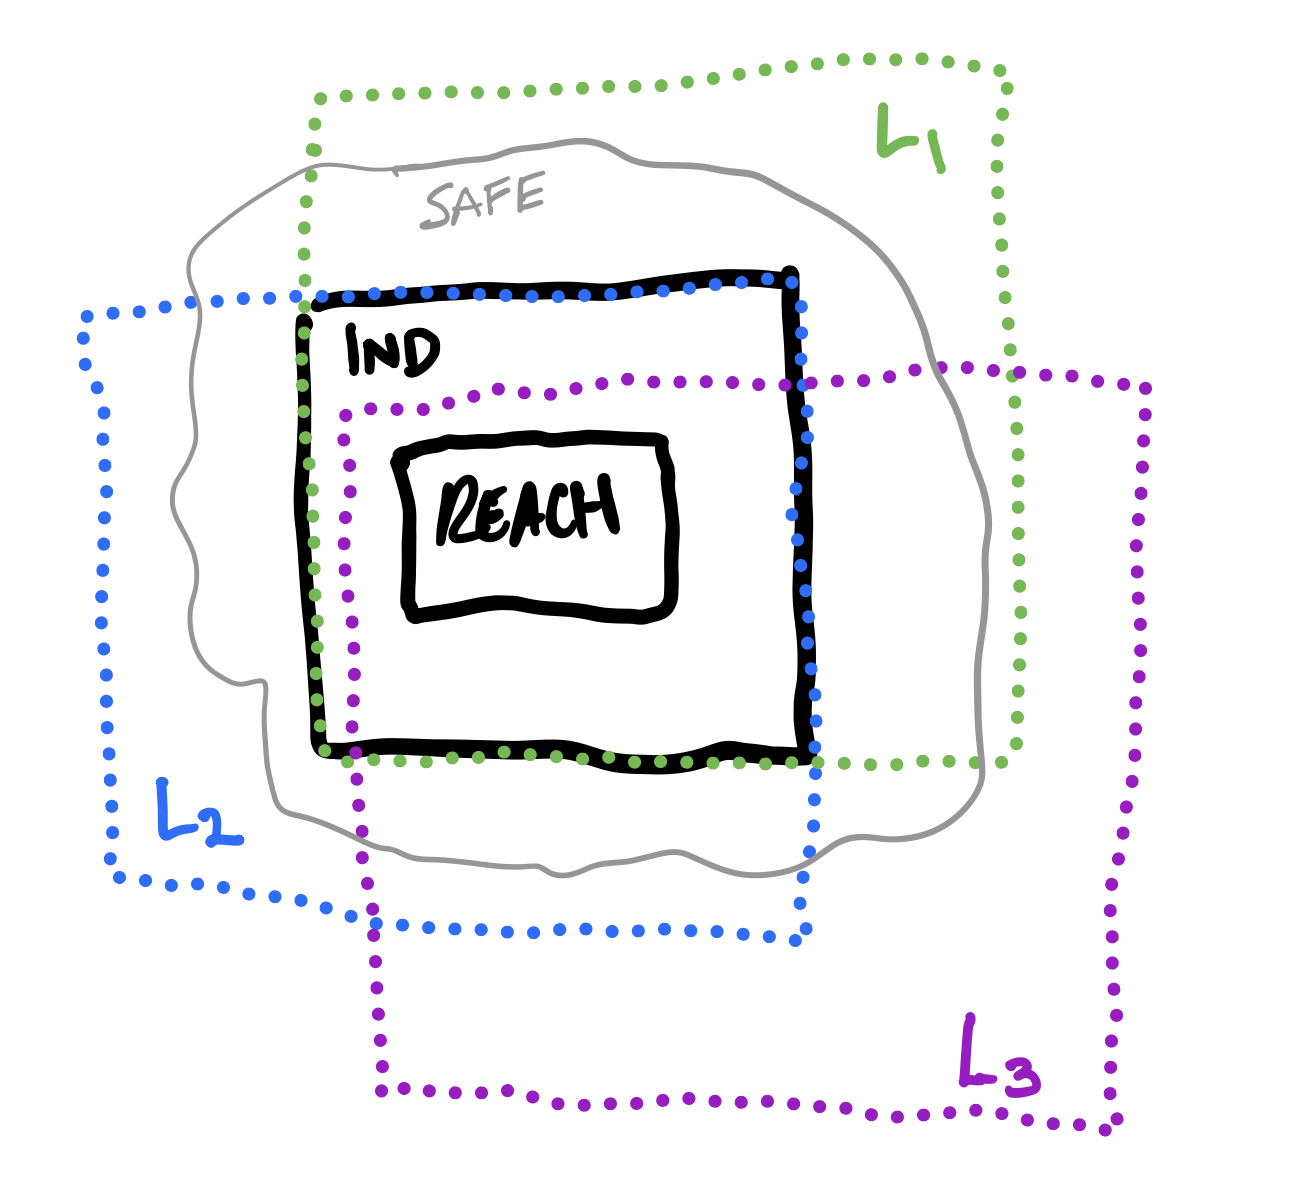
\includegraphics[width=70mm]{invs1.png}  
\end{center}

There are 3 invariants in our domain, $L_1,L_2,L_3$. If we select invariants in some order, are we guaranteed to converge to an inductive invariant? If we select $L_1$ and then $L_2$, then we will converge to $Ind$. But, if we select $L_1$ and then $L_3$, we will end up with a resulting predicate $L_1 \wedge L_3$ that is stronger than $Ind$, and we end up stuck, since there are no inductive ivnariants stronger than $Ind$ that are expressible in our abstraction domain. So, if we follow a strategy of strict refinement (always combining via conjunction), then we are inevitably stuck in this case. We could potentially undo a past choice, however, and try a different invariant selection strategy, in the style of standard backtracking search. But, a question is how to detect when we end up in this "dead end" refinement scenario.

If an inductive invariant exists that is representable in a given abstraction domain, will counterexample guided invariant search always find it?

We can say that our abstraction domain consists of the set of all invariants expressible by some given grammar. Then, we want to ask whether by selecting invariants in some manner, is it always possible we will learn

\begin{itemize}
    \item If you start off with a fixed abstraction domain, is there a way to dynamically adjust the domain if you realize that it cannot express the concepts (e.g. invariants) you want to express?
\end{itemize}







% \bibliographystyle{plain}
% \bibliography{../../references.bib}

% \printbibliography

\end{document}